\documentclass[14pt]{extbook}
\usepackage{multicol, enumerate, enumitem, hyperref, color, soul, setspace, parskip, fancyhdr} %General Packages
\usepackage{amssymb, amsthm, amsmath, latexsym, units, mathtools} %Math Packages
\everymath{\displaystyle} %All math in Display Style
% Packages with additional options
\usepackage[headsep=0.5cm,headheight=12pt, left=1 in,right= 1 in,top= 1 in,bottom= 1 in]{geometry}
\usepackage[usenames,dvipsnames]{xcolor}
\usepackage{dashrule}  % Package to use the command below to create lines between items
\newcommand{\litem}[1]{\item#1\hspace*{-1cm}\rule{\textwidth}{0.4pt}}
\pagestyle{fancy}
\lhead{Progress Quiz 4}
\chead{}
\rhead{Version ALL}
\lfoot{5346-5907}
\cfoot{}
\rfoot{Summer C 2021}
\begin{document}

\begin{enumerate}
\litem{
Solve the linear equation below. Then, choose the interval that contains the solution.\[ \frac{4x + 9}{3} - \frac{7x -6}{5} = \frac{-6x -6}{7} \]\begin{enumerate}[label=\Alph*.]
\item \( x \in [-6.7, -5.3] \)
\item \( x \in [-28.2, -25.3] \)
\item \( x \in [-3.2, -0.8] \)
\item \( x \in [-5.2, -2.7] \)
\item \( \text{There are no real solutions.} \)

\end{enumerate} }
\litem{
Solve the equation below. Then, choose the interval that contains the solution.\[ -12(-19x -11) = -18(-2x -5) \]\begin{enumerate}[label=\Alph*.]
\item \( x \in [-1.21, -0.9] \)
\item \( x \in [-0.86, -0.65] \)
\item \( x \in [0.48, 2.61] \)
\item \( x \in [-0.31, 0.24] \)
\item \( \text{There are no real solutions.} \)

\end{enumerate} }
\litem{
First, find the equation of the line containing the two points below. Then, write the equation in the form $ y=mx+b $ and choose the intervals that contain $m$ and $b$.\[ (7, -4) \text{ and } (-11, -10) \]\begin{enumerate}[label=\Alph*.]
\item \( m \in [-0.02, 1.47] \hspace*{3mm} b \in [4.33, 9.33] \)
\item \( m \in [-0.02, 1.47] \hspace*{3mm} b \in [-9.33, -2.33] \)
\item \( m \in [-0.79, 0.15] \hspace*{3mm} b \in [-17.67, -12.67] \)
\item \( m \in [-0.02, 1.47] \hspace*{3mm} b \in [-2, 3] \)
\item \( m \in [-0.02, 1.47] \hspace*{3mm} b \in [-13, -9] \)

\end{enumerate} }
\litem{
Write the equation of the line in the graph below in Standard Form $Ax+By=C$. Then, choose the intervals that contain $A, B, \text{ and } C$.
\begin{center}
    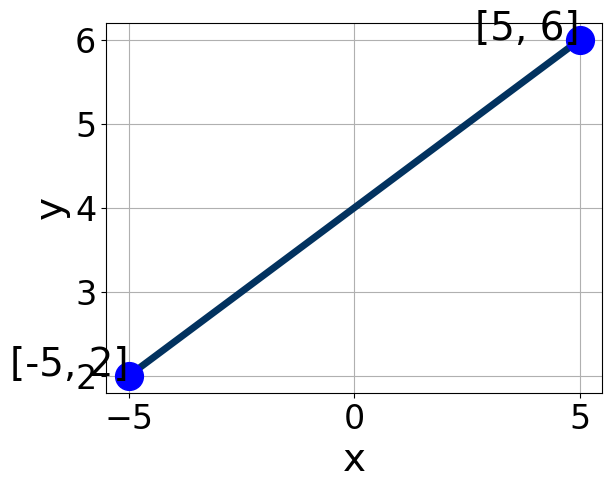
\includegraphics[width=0.5\textwidth]{../Figures/linearGraphToStandardCopyA.png}
\end{center}
\begin{enumerate}[label=\Alph*.]
\item \( A \in [-0.54, 0.83], \hspace{3mm} B \in [0.4, 1.3], \text{ and } \hspace{3mm} C \in [1, 5] \)
\item \( A \in [1.84, 2.92], \hspace{3mm} B \in [1.7, 6.9], \text{ and } \hspace{3mm} C \in [16, 28] \)
\item \( A \in [1.84, 2.92], \hspace{3mm} B \in [-5.6, -4.3], \text{ and } \hspace{3mm} C \in [-20, -14] \)
\item \( A \in [-0.54, 0.83], \hspace{3mm} B \in [-4.4, -0.7], \text{ and } \hspace{3mm} C \in [-8, -2] \)
\item \( A \in [-2.65, -1.44], \hspace{3mm} B \in [1.7, 6.9], \text{ and } \hspace{3mm} C \in [16, 28] \)

\end{enumerate} }
\litem{
Find the equation of the line described below. Write the linear equation in the form $ y=mx+b $ and choose the intervals that contain $m$ and $b$.\[ \text{Perpendicular to } 7 x + 9 y = 9 \text{ and passing through the point } (-7, -3). \]\begin{enumerate}[label=\Alph*.]
\item \( m \in [1.23, 2.14] \hspace*{3mm} b \in [5.2, 7.1] \)
\item \( m \in [1.23, 2.14] \hspace*{3mm} b \in [3.3, 4.4] \)
\item \( m \in [1.23, 2.14] \hspace*{3mm} b \in [-6.7, -2.7] \)
\item \( m \in [-1.31, -0.88] \hspace*{3mm} b \in [-15, -11.4] \)
\item \( m \in [0.52, 0.95] \hspace*{3mm} b \in [5.2, 7.1] \)

\end{enumerate} }
\litem{
Solve the equation below. Then, choose the interval that contains the solution.\[ -13(-16x -3) = -2(-6x -19) \]\begin{enumerate}[label=\Alph*.]
\item \( x \in [-0.01, 0.04] \)
\item \( x \in [-0.41, -0.38] \)
\item \( x \in [-0.35, -0.34] \)
\item \( x \in [0.39, 0.42] \)
\item \( \text{There are no real solutions.} \)

\end{enumerate} }
\litem{
Find the equation of the line described below. Write the linear equation in the form $ y=mx+b $ and choose the intervals that contain $m$ and $b$.\[ \text{Parallel to } 9 x + 7 y = 13 \text{ and passing through the point } (-6, -6). \]\begin{enumerate}[label=\Alph*.]
\item \( m \in [-1.36, -0.79] \hspace*{3mm} b \in [7.71, 16.71] \)
\item \( m \in [-1.36, -0.79] \hspace*{3mm} b \in [-14.71, -10.71] \)
\item \( m \in [-0.92, 0.06] \hspace*{3mm} b \in [-14.71, -10.71] \)
\item \( m \in [1.21, 1.32] \hspace*{3mm} b \in [1.71, 6.71] \)
\item \( m \in [-1.36, -0.79] \hspace*{3mm} b \in [-3, 1] \)

\end{enumerate} }
\litem{
Write the equation of the line in the graph below in Standard Form $Ax+By=C$. Then, choose the intervals that contain $A, B, \text{ and } C$.
\begin{center}
    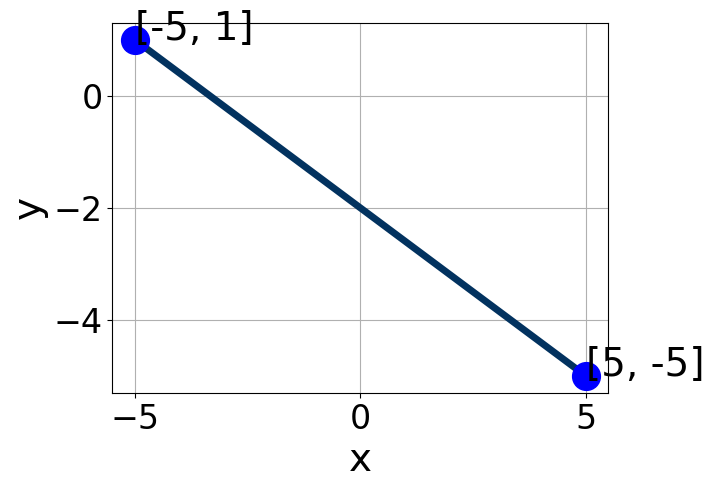
\includegraphics[width=0.5\textwidth]{../Figures/linearGraphToStandardA.png}
\end{center}
\begin{enumerate}[label=\Alph*.]
\item \( A \in [-2.4, 2.6], \hspace{3mm} B \in [-0.4, 1.8], \text{ and } \hspace{3mm} C \in [-2, 0] \)
\item \( A \in [1, 6], \hspace{3mm} B \in [2.9, 5.2], \text{ and } \hspace{3mm} C \in [-15, -7] \)
\item \( A \in [-8, -2], \hspace{3mm} B \in [-5.8, -4.3], \text{ and } \hspace{3mm} C \in [10, 12] \)
\item \( A \in [-2.4, 2.6], \hspace{3mm} B \in [-4, -0.7], \text{ and } \hspace{3mm} C \in [2, 3] \)
\item \( A \in [1, 6], \hspace{3mm} B \in [-5.8, -4.3], \text{ and } \hspace{3mm} C \in [10, 12] \)

\end{enumerate} }
\litem{
Solve the linear equation below. Then, choose the interval that contains the solution.\[ \frac{-4x -7}{8} - \frac{4x + 4}{3} = \frac{-4x + 9}{4} \]\begin{enumerate}[label=\Alph*.]
\item \( x \in [-25.1, -22.8] \)
\item \( x \in [-3.9, -1.2] \)
\item \( x \in [-1.5, 0.2] \)
\item \( x \in [-6.2, -4.7] \)
\item \( \text{There are no real solutions.} \)

\end{enumerate} }
\litem{
First, find the equation of the line containing the two points below. Then, write the equation in the form $ y=mx+b $ and choose the intervals that contain $m$ and $b$.\[ (8, -5) \text{ and } (-7, -6) \]\begin{enumerate}[label=\Alph*.]
\item \( m \in [0.05, 0.24] \hspace*{3mm} b \in [-5.7, -3.4] \)
\item \( m \in [0.05, 0.24] \hspace*{3mm} b \in [-0.7, 2.9] \)
\item \( m \in [-0.22, 0.02] \hspace*{3mm} b \in [-7.4, -6.1] \)
\item \( m \in [0.05, 0.24] \hspace*{3mm} b \in [3.5, 7.5] \)
\item \( m \in [0.05, 0.24] \hspace*{3mm} b \in [-14.3, -12.7] \)

\end{enumerate} }
\litem{
Solve the linear equation below. Then, choose the interval that contains the solution.\[ \frac{3x -7}{3} - \frac{-3x + 5}{8} = \frac{4x + 9}{5} \]\begin{enumerate}[label=\Alph*.]
\item \( x \in [3.1, 8.1] \)
\item \( x \in [35.52, 40.52] \)
\item \( x \in [1.38, 3.38] \)
\item \( x \in [7.28, 10.28] \)
\item \( \text{There are no real solutions.} \)

\end{enumerate} }
\litem{
Solve the equation below. Then, choose the interval that contains the solution.\[ -6(18x -19) = -17(15x -4) \]\begin{enumerate}[label=\Alph*.]
\item \( x \in [0.61, 2.22] \)
\item \( x \in [-0.62, 0.21] \)
\item \( x \in [-0.07, 0.74] \)
\item \( x \in [-1.89, -1.23] \)
\item \( \text{There are no real solutions.} \)

\end{enumerate} }
\litem{
First, find the equation of the line containing the two points below. Then, write the equation in the form $ y=mx+b $ and choose the intervals that contain $m$ and $b$.\[ (9, -4) \text{ and } (5, 9) \]\begin{enumerate}[label=\Alph*.]
\item \( m \in [-1.75, 6.25] \hspace*{3mm} b \in [-11.25, -5.25] \)
\item \( m \in [-4.25, -2.25] \hspace*{3mm} b \in [-18, -8] \)
\item \( m \in [-4.25, -2.25] \hspace*{3mm} b \in [-1, 8] \)
\item \( m \in [-4.25, -2.25] \hspace*{3mm} b \in [-33.25, -24.25] \)
\item \( m \in [-4.25, -2.25] \hspace*{3mm} b \in [24.25, 31.25] \)

\end{enumerate} }
\litem{
Write the equation of the line in the graph below in Standard Form $Ax+By=C$. Then, choose the intervals that contain $A, B, \text{ and } C$.
\begin{center}
    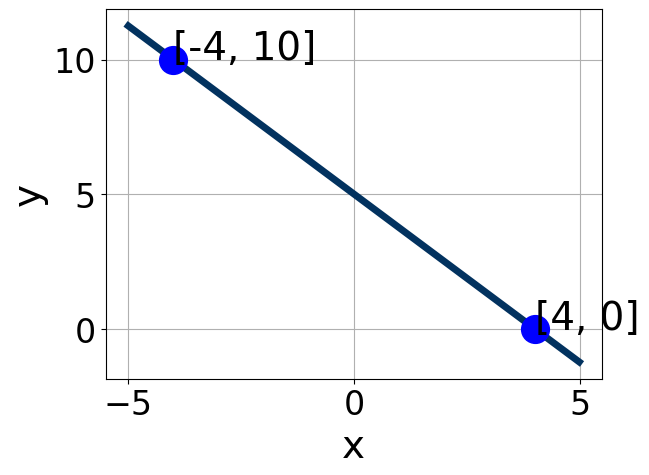
\includegraphics[width=0.5\textwidth]{../Figures/linearGraphToStandardCopyB.png}
\end{center}
\begin{enumerate}[label=\Alph*.]
\item \( A \in [4.7, 7.3], \hspace{3mm} B \in [2.94, 4.93], \text{ and } \hspace{3mm} C \in [18, 26] \)
\item \( A \in [-0.2, 2.9], \hspace{3mm} B \in [0.43, 1.51], \text{ and } \hspace{3mm} C \in [-1, 6] \)
\item \( A \in [-0.2, 2.9], \hspace{3mm} B \in [-2.57, 0.34], \text{ and } \hspace{3mm} C \in [-9, -2] \)
\item \( A \in [-8.8, -4.1], \hspace{3mm} B \in [-4.81, -3.18], \text{ and } \hspace{3mm} C \in [-20, -17] \)
\item \( A \in [4.7, 7.3], \hspace{3mm} B \in [-4.81, -3.18], \text{ and } \hspace{3mm} C \in [-20, -17] \)

\end{enumerate} }
\litem{
Find the equation of the line described below. Write the linear equation in the form $ y=mx+b $ and choose the intervals that contain $m$ and $b$.\[ \text{Perpendicular to } 6 x + 7 y = 8 \text{ and passing through the point } (6, 8). \]\begin{enumerate}[label=\Alph*.]
\item \( m \in [0.24, 0.9] \hspace*{3mm} b \in [0.27, 1.74] \)
\item \( m \in [-1.49, -0.49] \hspace*{3mm} b \in [14.55, 16.43] \)
\item \( m \in [1.03, 1.47] \hspace*{3mm} b \in [0.27, 1.74] \)
\item \( m \in [1.03, 1.47] \hspace*{3mm} b \in [-1.21, -0.14] \)
\item \( m \in [1.03, 1.47] \hspace*{3mm} b \in [1.71, 2.97] \)

\end{enumerate} }
\litem{
Solve the equation below. Then, choose the interval that contains the solution.\[ -19(7x -12) = -2(11x -5) \]\begin{enumerate}[label=\Alph*.]
\item \( x \in [-2.29, -2.1] \)
\item \( x \in [2.13, 2.41] \)
\item \( x \in [1.91, 2.08] \)
\item \( x \in [1.43, 1.61] \)
\item \( \text{There are no real solutions.} \)

\end{enumerate} }
\litem{
Find the equation of the line described below. Write the linear equation in the form $ y=mx+b $ and choose the intervals that contain $m$ and $b$.\[ \text{Perpendicular to } 8 x - 7 y = 10 \text{ and passing through the point } (2, -2). \]\begin{enumerate}[label=\Alph*.]
\item \( m \in [-1, -0.2] \hspace*{3mm} b \in [-4.1, -3.8] \)
\item \( m \in [0.4, 1] \hspace*{3mm} b \in [-3.88, -3.55] \)
\item \( m \in [-1, -0.2] \hspace*{3mm} b \in [-0.03, 0.46] \)
\item \( m \in [-1, -0.2] \hspace*{3mm} b \in [-0.3, 0.01] \)
\item \( m \in [-2.3, -1] \hspace*{3mm} b \in [-0.3, 0.01] \)

\end{enumerate} }
\litem{
Write the equation of the line in the graph below in Standard Form $Ax+By=C$. Then, choose the intervals that contain $A, B, \text{ and } C$.
\begin{center}
    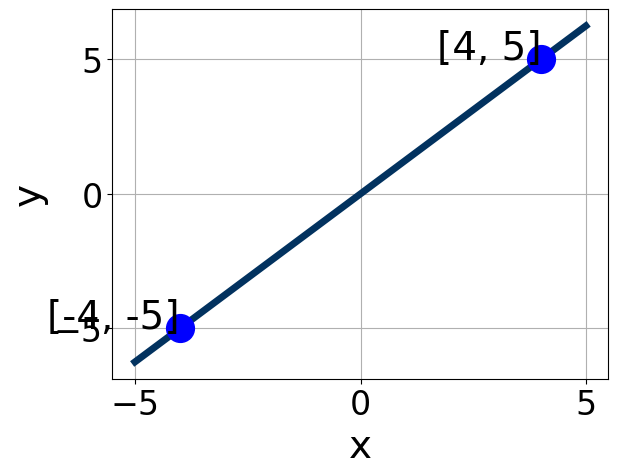
\includegraphics[width=0.5\textwidth]{../Figures/linearGraphToStandardB.png}
\end{center}
\begin{enumerate}[label=\Alph*.]
\item \( A \in [4, 7.2], \hspace{3mm} B \in [-4.7, -3.4], \text{ and } \hspace{3mm} C \in [-1, 7] \)
\item \( A \in [-5.9, -3.7], \hspace{3mm} B \in [3.6, 6.8], \text{ and } \hspace{3mm} C \in [-1, 7] \)
\item \( A \in [-2.1, 2.8], \hspace{3mm} B \in [-1.7, -0.2], \text{ and } \hspace{3mm} C \in [-1, 7] \)
\item \( A \in [4, 7.2], \hspace{3mm} B \in [3.6, 6.8], \text{ and } \hspace{3mm} C \in [-1, 7] \)
\item \( A \in [-2.1, 2.8], \hspace{3mm} B \in [-0.3, 2.7], \text{ and } \hspace{3mm} C \in [-1, 7] \)

\end{enumerate} }
\litem{
Solve the linear equation below. Then, choose the interval that contains the solution.\[ \frac{-7x -6}{3} - \frac{-9x -4}{4} = \frac{-7x + 8}{5} \]\begin{enumerate}[label=\Alph*.]
\item \( x \in [3.1, 5.8] \)
\item \( x \in [1.6, 2.2] \)
\item \( x \in [-0.1, 0.3] \)
\item \( x \in [6.9, 8] \)
\item \( \text{There are no real solutions.} \)

\end{enumerate} }
\litem{
First, find the equation of the line containing the two points below. Then, write the equation in the form $ y=mx+b $ and choose the intervals that contain $m$ and $b$.\[ (8, -11) \text{ and } (6, 9) \]\begin{enumerate}[label=\Alph*.]
\item \( m \in [-14, -1] \hspace*{3mm} b \in [2, 8] \)
\item \( m \in [6, 11] \hspace*{3mm} b \in [-52, -48] \)
\item \( m \in [-14, -1] \hspace*{3mm} b \in [-21, -12] \)
\item \( m \in [-14, -1] \hspace*{3mm} b \in [66, 73] \)
\item \( m \in [-14, -1] \hspace*{3mm} b \in [-73, -68] \)

\end{enumerate} }
\litem{
Solve the linear equation below. Then, choose the interval that contains the solution.\[ \frac{-7x + 6}{8} - \frac{5x -8}{2} = \frac{-5x -4}{7} \]\begin{enumerate}[label=\Alph*.]
\item \( x \in [0.1, 1.2] \)
\item \( x \in [1.7, 3.1] \)
\item \( x \in [-2.6, -0.4] \)
\item \( x \in [6.2, 8] \)
\item \( \text{There are no real solutions.} \)

\end{enumerate} }
\litem{
Solve the equation below. Then, choose the interval that contains the solution.\[ -19(14x + 6) = -3(4x -16) \]\begin{enumerate}[label=\Alph*.]
\item \( x \in [-0.77, -0.57] \)
\item \( x \in [-0.34, -0.25] \)
\item \( x \in [-0.25, -0.17] \)
\item \( x \in [0.18, 0.4] \)
\item \( \text{There are no real solutions.} \)

\end{enumerate} }
\litem{
First, find the equation of the line containing the two points below. Then, write the equation in the form $ y=mx+b $ and choose the intervals that contain $m$ and $b$.\[ (2, 8) \text{ and } (4, -2) \]\begin{enumerate}[label=\Alph*.]
\item \( m \in [-12, -4] \hspace*{3mm} b \in [4, 10] \)
\item \( m \in [-12, -4] \hspace*{3mm} b \in [-6, -2] \)
\item \( m \in [-12, -4] \hspace*{3mm} b \in [-20, -14] \)
\item \( m \in [4, 6] \hspace*{3mm} b \in [-26, -20] \)
\item \( m \in [-12, -4] \hspace*{3mm} b \in [17, 19] \)

\end{enumerate} }
\litem{
Write the equation of the line in the graph below in Standard Form $Ax+By=C$. Then, choose the intervals that contain $A, B, \text{ and } C$.
\begin{center}
    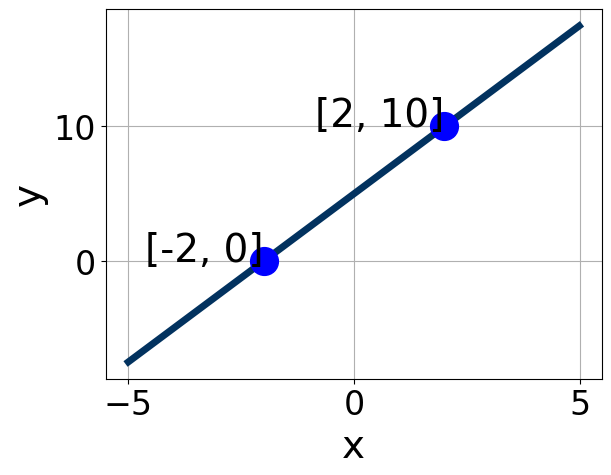
\includegraphics[width=0.5\textwidth]{../Figures/linearGraphToStandardCopyC.png}
\end{center}
\begin{enumerate}[label=\Alph*.]
\item \( A \in [-2.5, -1.5], \hspace{3mm} B \in [0.1, 1.11], \text{ and } \hspace{3mm} C \in [4, 7] \)
\item \( A \in [-6, -3], \hspace{3mm} B \in [1.49, 3.66], \text{ and } \hspace{3mm} C \in [9, 11] \)
\item \( A \in [-2.5, -1.5], \hspace{3mm} B \in [-1.41, -0.53], \text{ and } \hspace{3mm} C \in [-7, -4] \)
\item \( A \in [4, 8], \hspace{3mm} B \in [1.49, 3.66], \text{ and } \hspace{3mm} C \in [9, 11] \)
\item \( A \in [4, 8], \hspace{3mm} B \in [-3.93, -1.4], \text{ and } \hspace{3mm} C \in [-12, -7] \)

\end{enumerate} }
\litem{
Find the equation of the line described below. Write the linear equation in the form $ y=mx+b $ and choose the intervals that contain $m$ and $b$.\[ \text{Parallel to } 7 x - 8 y = 9 \text{ and passing through the point } (7, 8). \]\begin{enumerate}[label=\Alph*.]
\item \( m \in [0.77, 0.95] \hspace*{3mm} b \in [0.05, 1.77] \)
\item \( m \in [0.77, 0.95] \hspace*{3mm} b \in [-2.58, -0.48] \)
\item \( m \in [0.98, 1.67] \hspace*{3mm} b \in [1.55, 2.01] \)
\item \( m \in [-1.19, -0.36] \hspace*{3mm} b \in [13.58, 15.14] \)
\item \( m \in [0.77, 0.95] \hspace*{3mm} b \in [1.55, 2.01] \)

\end{enumerate} }
\litem{
Solve the equation below. Then, choose the interval that contains the solution.\[ -13(17x -2) = -12(-9x -4) \]\begin{enumerate}[label=\Alph*.]
\item \( x \in [0.65, 0.74] \)
\item \( x \in [-0.28, -0.21] \)
\item \( x \in [-0.18, 0.14] \)
\item \( x \in [0.03, 0.28] \)
\item \( \text{There are no real solutions.} \)

\end{enumerate} }
\litem{
Find the equation of the line described below. Write the linear equation in the form $ y=mx+b $ and choose the intervals that contain $m$ and $b$.\[ \text{Parallel to } 5 x - 4 y = 4 \text{ and passing through the point } (-8, 5). \]\begin{enumerate}[label=\Alph*.]
\item \( m \in [1.14, 1.98] \hspace*{3mm} b \in [14, 18] \)
\item \( m \in [-2, -0.92] \hspace*{3mm} b \in [-9, -1] \)
\item \( m \in [1.14, 1.98] \hspace*{3mm} b \in [-16, -12] \)
\item \( m \in [0.37, 0.85] \hspace*{3mm} b \in [14, 18] \)
\item \( m \in [1.14, 1.98] \hspace*{3mm} b \in [10, 14] \)

\end{enumerate} }
\litem{
Write the equation of the line in the graph below in Standard Form $Ax+By=C$. Then, choose the intervals that contain $A, B, \text{ and } C$.
\begin{center}
    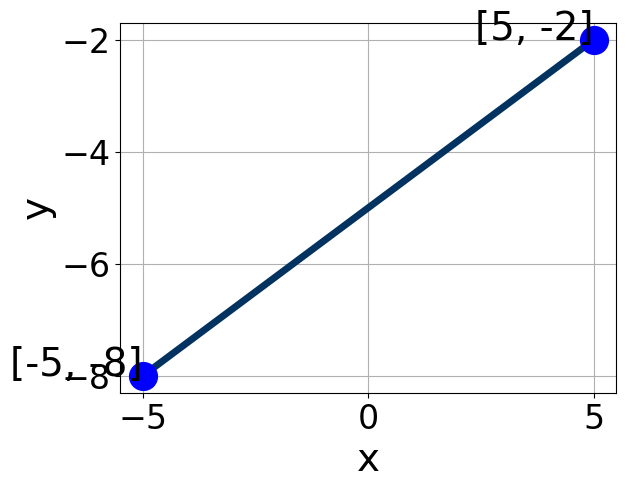
\includegraphics[width=0.5\textwidth]{../Figures/linearGraphToStandardC.png}
\end{center}
\begin{enumerate}[label=\Alph*.]
\item \( A \in [-7.6, -1.2], \hspace{3mm} B \in [1.2, 5.1], \text{ and } \hspace{3mm} C \in [-29, -23] \)
\item \( A \in [-1.1, 1.2], \hspace{3mm} B \in [-2, -0.4], \text{ and } \hspace{3mm} C \in [4, 6] \)
\item \( A \in [2.1, 5.6], \hspace{3mm} B \in [-5.8, -2.8], \text{ and } \hspace{3mm} C \in [19, 34] \)
\item \( A \in [2.1, 5.6], \hspace{3mm} B \in [1.2, 5.1], \text{ and } \hspace{3mm} C \in [-29, -23] \)
\item \( A \in [-1.1, 1.2], \hspace{3mm} B \in [-0.7, 1.5], \text{ and } \hspace{3mm} C \in [-10, 2] \)

\end{enumerate} }
\litem{
Solve the linear equation below. Then, choose the interval that contains the solution.\[ \frac{-8x + 8}{3} - \frac{-8x -8}{5} = \frac{-8x + 7}{4} \]\begin{enumerate}[label=\Alph*.]
\item \( x \in [-0.6, 0.1] \)
\item \( x \in [-10.2, -7.4] \)
\item \( x \in [-3.2, -2.2] \)
\item \( x \in [0.5, 1.1] \)
\item \( \text{There are no real solutions.} \)

\end{enumerate} }
\litem{
First, find the equation of the line containing the two points below. Then, write the equation in the form $ y=mx+b $ and choose the intervals that contain $m$ and $b$.\[ (-3, 10) \text{ and } (-7, -9) \]\begin{enumerate}[label=\Alph*.]
\item \( m \in [-0.25, 6.75] \hspace*{3mm} b \in [10, 21] \)
\item \( m \in [-0.25, 6.75] \hspace*{3mm} b \in [-31.25, -22.25] \)
\item \( m \in [-0.25, 6.75] \hspace*{3mm} b \in [-7, 2] \)
\item \( m \in [-0.25, 6.75] \hspace*{3mm} b \in [23.25, 25.25] \)
\item \( m \in [-4.75, 1.25] \hspace*{3mm} b \in [-42.25, -40.25] \)

\end{enumerate} }
\end{enumerate}

\end{document}